\chapter{Introduction} \label{chapter:intro}
\section{Background} %fd
Autonomous driving has seen an explosion of research in academia and industry. Most of these efforts focus on studying scenarios and control in urban environments such as day-to-day driving on streets and highways. However, there is growing interest towards incorporating autonomy in motorsports. Many advancements in commercial automobiles have originated from projects invented for use in motorsports such as traction control, energy recovery systems, and sequential gearboxes (CITE THIS). 

Modeling an autonomous racing game is inherently similar to an urban driving scenario. For example, they are both focused on controlling four-wheeled automobiles. The primary objective of the drivers is to reach some destination in the shortest time. In racing, however, the interactions between the players are more aggressive because there is an additional nuance in objective to finish ahead of other players. Racing and urban driving also both involve complex rules governing the interactions amongst the players. In both contexts, these rules are primarily designed to ensure everyone's safety, but the difference between the between the contexts relates to the extent of the rules. Depending on the situation, we have different answers to questions such as: ``how fast is everyone allowed to go?" or ``what is the minimum distance required to be maintained between the cars?". All of these contrasts between racing and urban driving relate to the motivation of participating in a racing game, which is to explore the limits of performance. Therefore, studying autonomous racing is an opportunity to develop autonomous driving controllers to be highly-performant, robust and safe in challenging scenarios. 

Finally, in addition to pushing the boundaries of autonomous driving algorithms, researching autonomous racing also paves way for developing simulators to train human drivers. Motorsport teams already spend millions of dollars developing highly sophisticated simulators to train their drivers to become experts at driving around a track that may not even be fully constructed (CITE THIS). If they start including simluations of opponents who follow the rules of racing but also provide the precise control of a computer, the teams' drivers can learn what kind of strategies are viable and practice specific scenarios for hours without burning a single drop of fuel.

\section{Motivation} %td
Most prior research in autonomous racing controllers generally relies on model predictive control methods. As name suggests, the general structure of these approaches is to solve optimization problems with nonlinear dynamics constraints and objectives. This type of calculation is limited a short time horizon (1-3 seconds) because the problem must be simple enough to solve at rates of 20-30 times a second even with state-of-the-art tools. 

\begin{figure}
\begin{center}
   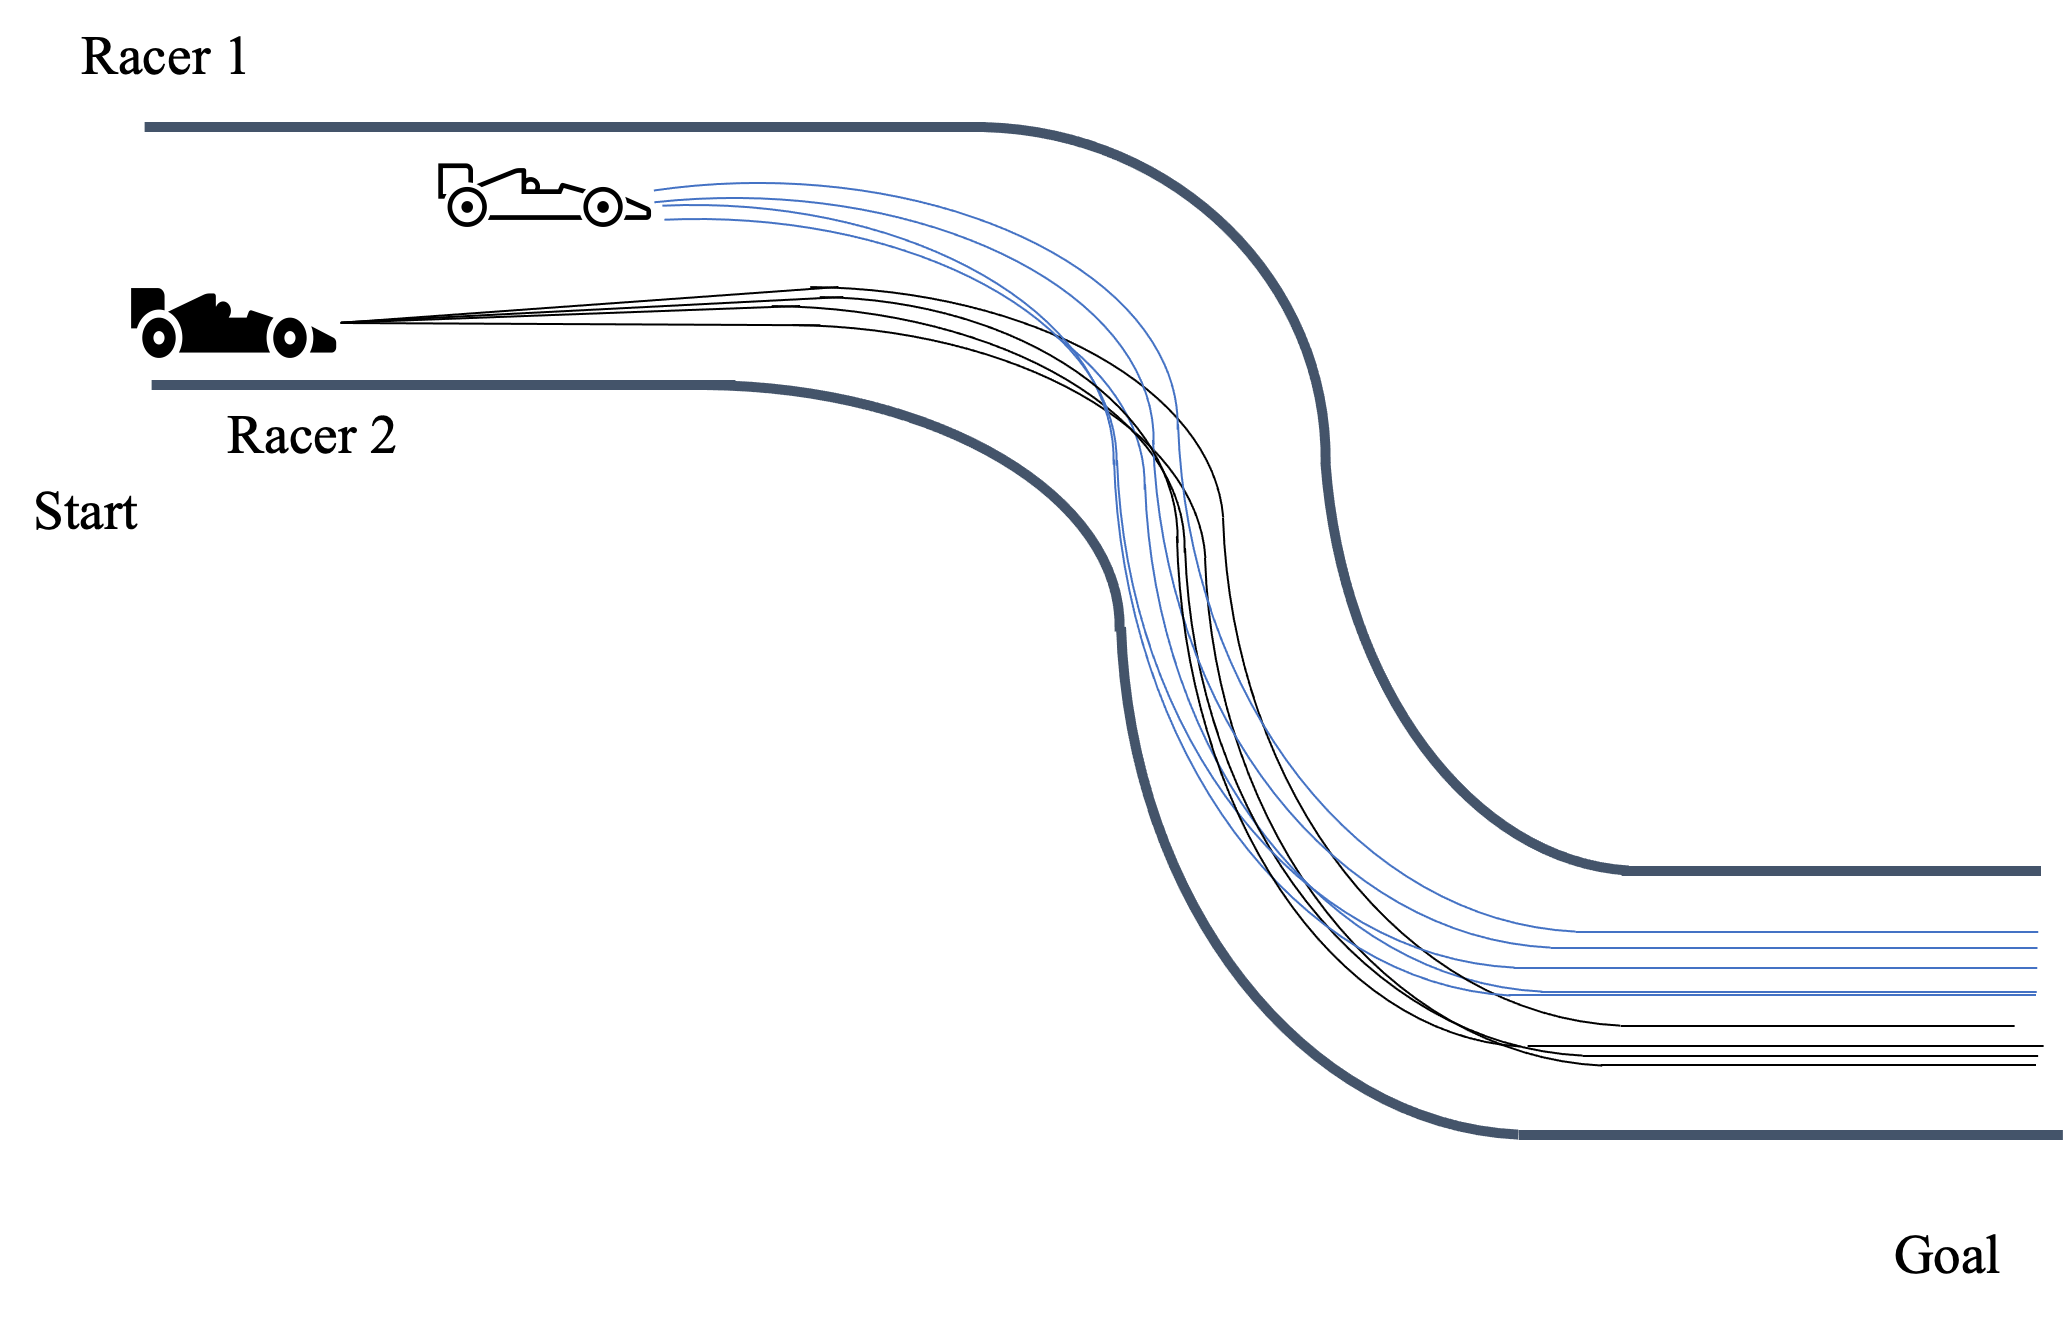
\includegraphics[width=0.75\textwidth]{Figures/MotivatingExampleInfTraj.png}
\caption{Uncountably infinite trajectories to consider in racing.}
\label{fig:motivating_example:inf}
\end{center}
\end{figure}

In addition, prior work is also mainly focused on single-agent control or situations with agents who behave as stationary or dynamic obstacles rather than adversaries (CITE THIS). However, when we hear the term ``racing," we naturally think of it as multi-agent game where all participants are competing against one another. Although it is possible to introduce adversarial objectives and constraints in the optimization-based control methods, they are prone to computational limitations in terms of planning horizon or control frequency for direct low-level control (CITE THIS). Consider the simple scenario in Figure \ref{fig:motivating_example:inf}. There is an infinite number of trajectories that the black car could use to overtake the white car across the next two turns on a track. In order to use existing methods, we must compromise by either shortening the planning horizon and/or simplifying the objectives or constraints in the model. With a short horizon, it is just infeasible to plan for the medium-term to long-term strategic decisions to successfully overtake. Otherwise, if the model is simplified, we may no longer have an accurate representation of the game's rules or dynamics. With either compromise we lose the ability to perform the long-term game theoretic reasoning.

\begin{figure}
\begin{center}
   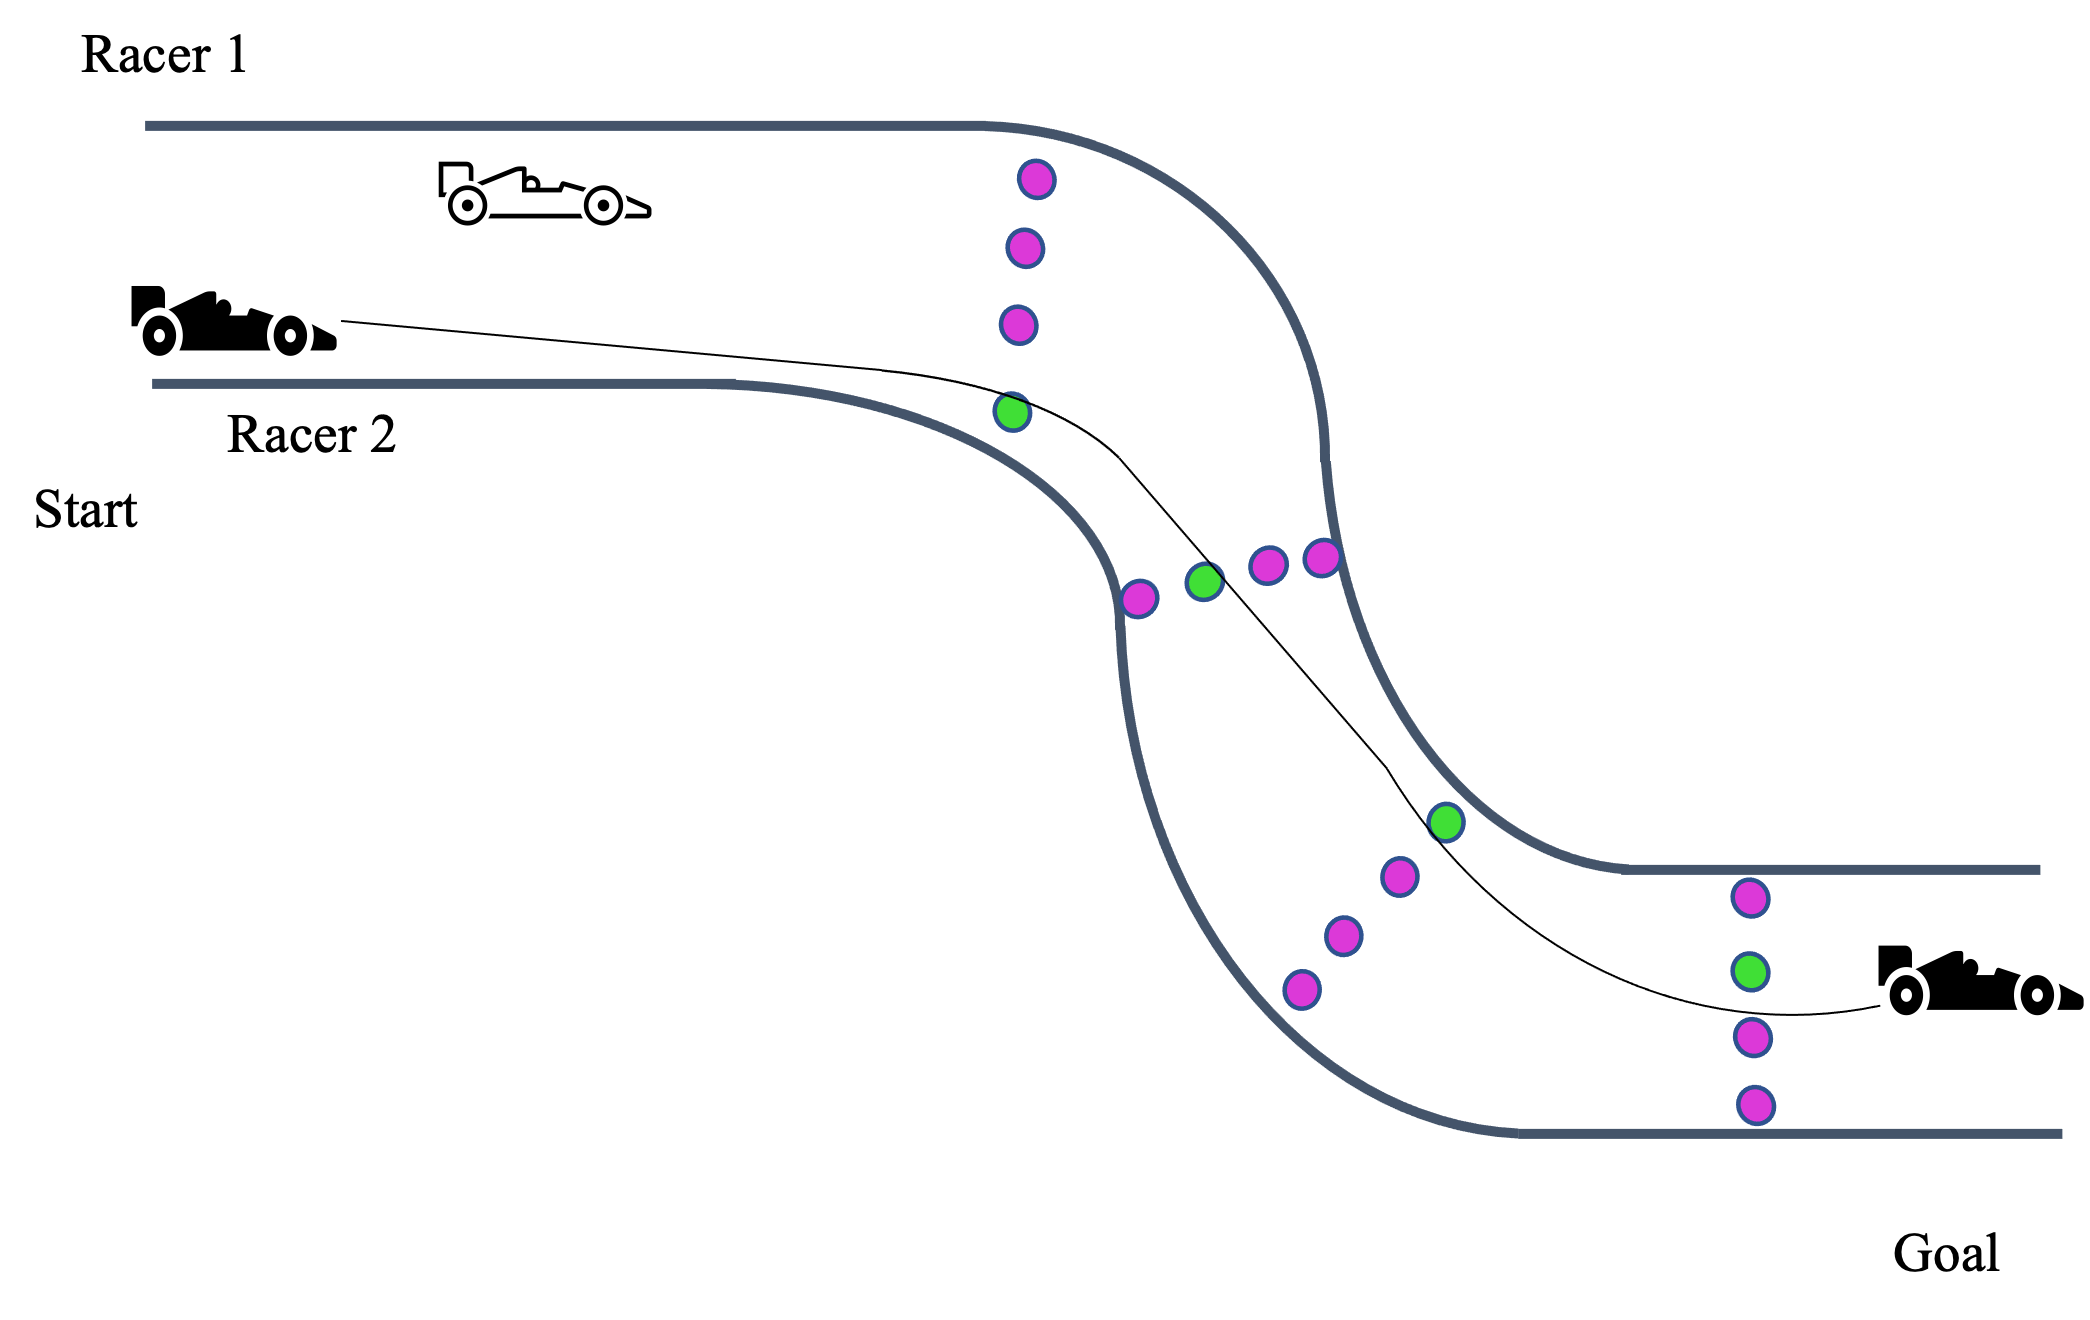
\includegraphics[width=0.75\textwidth]{Figures/MotivatingExampleOracle.png}
\caption{A high-level plan outlining lane choices (green) followed by a single trajectory (black).}
\label{fig:motivating_example:oracle}
\end{center}
\end{figure}

Therefore, practical implementation of such a complex control application suggests breaking down the system into layers of hierarchical reasoning (Figure \ref{fig:motivating_example:oracle}). There are effectively four high-level decisions to make in this scenario located at the first turn entry, the first turn exit the second turn entry, and the second turn exit. The domain of these decisions involves determining which of the four lanes to be positioned at each of the locations. If there is an oracle that can determine the ideal choice of lane for those locations such that the rules and dynamics are satisfied, highlighted in green, the problem for our precise, low-level controller becomes much simpler. It no longer needs to decide both where to be positioned and how to move between those positions; rather, is just a matter of calculating the latter. 

\section{Contributions} %td
This report develops a hierarchical control scheme that reasons about optimal long-term plans and adheres to the safety and fairness rules seen in real-life multi-agent racing. We provide a general formulation for a multi-agent racing game that encodes these complex rules and study the problem in three parts.

In the first part, we construct a turn-based, discrete simplification of a racing game that encapsulates the discrete nature of the safety and fairness rules from the general formulation. We outline temporal logic specifications to represent these rules and use the specifications to rule out players' choices in the game. Furthermore, we develop a turn-based mechanism to preserve the realistic flow of information that would occur in a continuous setting. Our resulting discrete game has a simple reachability objective over a finite number of steps, which is solved using value iteration. We evaluate our formulation by considering three case studies of common racing scenarios. 

In the second part, we use construct the full hierarchical control scheme for head-to-head racing that runs in real-time. We use the discrete game formulation from the first part as the high-level planner and use Monte Carlo tree search to solve the game in real-time. The solution of the discrete formulation effectively produces a series of long-term waypoints that are safe with respect to the rules and approximately optimal. Then, we formulate a simplified version of the general racing game to track the waypoints with relaxed representations of the original rules. The simplified game is solved using two methods to produce high-resolution control inputs: training a policy using multi-agent reinforcement learning and solving a linear-quadratic Nash game approximation. Our structure yields a pair of hierarchical controllers that run in real-time and outperform baselines resembling previously studied autonomous racing methods in terms of head-to-head performance and obedience for following safety rules. Moreover, our controllers produce behavior resembling that of expert human drivers. 

In the final part, we consider an extension of head-to-head racing by introducing team-based objectives, which is a major part of real-life competitions. To our knowledge, this is one of only two works to study a mix of cooperative and competitive objectives in multi-agent racing. We generalize each of our game formulations from the previous sections by updating the objectives to evaluate the performance of one or more players on a team while subject to the same rules and constraints. Then, we use our proposed hierarchical control structure and compare them with the baseline methods adapted to play the updated form of the game. Our controllers show impressive performance compared to the baselines although the game has become more complex. Again, our controllers exhibit tactics resembling human experts.

Although this hierarchical control method is developed in the context of a racing game, the structure of the proposed architecture effectively reasons about optimal choices in a game-theoretic setting with complex constraints involving temporal logic and both continuous and discrete dynamics. As a result, we can apply this method to many other competitive settings that exhibit the aforementioned properties such as financial systems, power systems, or traffic control systems.

\section{Outline}
The remainder of this report is organized as follows. 
% Chapter \ref{chapter:prelim} summarizes some preliminaries for this report. 
Chapter \ref{chapter:litreview} provides a literature review of prior research in autonomous racing. 
Chapter \ref{chapter:synthesis} introduces the general racing game formulation, and outlines the discrete game abstraction of the general formulation. 
Chapter \ref{chapter:hier} develops the full hierarchical control scheme by utilizing the discrete formulation from the previous chapter as a high-level planner and constructing low-level formulation. 
Chapter \ref{chapter:team} applies the hierarchical controller to a team-based multi-agent racing. 
Finally, Chapter \ref{chapter:conclusion} concludes this work by providing a summary and ideas for further extensions. 